\documentclass[9pt,conference]{IEEEtran}
\usepackage[utf8]{inputenc}
\usepackage[brazil]{babel}

% Diversos
\usepackage{csquotes}
\usepackage{graphicx}
\usepackage{verbatim}
\usepackage{hyperref}
\usepackage{smartdiagram}

% Título
\title{Utilizando Redes Convolucionais de Grafos Espaço-Temporais para o Reconhecimento da Línguas de Sinais}
%\author{Cleison Correia de Amorim}
\date{Outubro 2018}

\author{
    \IEEEauthorblockN{Cleison Correia de Amorim}
    \IEEEauthorblockA{Centro de Informática\\
    Universidade Federal de Pernambuco\\
    Email: cca5@cin.ufpe.br}
}

% Comandos
% 'image': definição de imagem
\newcommand{\image}[4][\linewidth] {
    \begin{figure}[ht]
    \centering
    \includegraphics[width=#1]{#3}
    \caption{#4}
    \label{#2}
    \end{figure}
}

% 'refimage': referências de imagens
\newcommand{\refimage}[1] {figura \ref{#1}}

% 'refsection': referências de seções
\newcommand{\refsect}[1] {seção "\nameref{#1}"}


\begin{document}

\maketitle

\section{Introdução}
There is a theory which states that if ever anyone discovers exactly what the Universe is for and why it is here, it will instantly disappear and be replaced by something even more bizarre and inexplicable.
There is another theory which states that this has already happened.

\begin{figure}[h!]
\centering
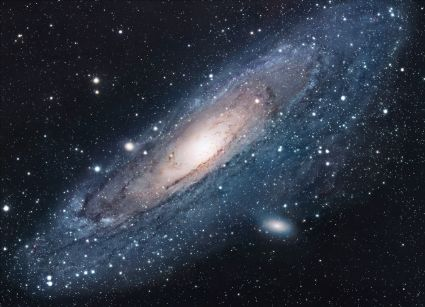
\includegraphics[scale=1.7]{images/universe}
\caption{The Universe}
\label{fig:universe}
\end{figure}

\section{Conclusion}
``I always thought something was fundamentally wrong with the universe'' \citep{adams1995hitchhiker}

\bibliographystyle{plain}
\bibliography{references}
\end{document}
